% ============================================================
%  深圳大学实验报告 - Project: Blog Application Design
% ============================================================

\documentclass[a4paper,12pt]{article}

% ----------------------------
% 宏包与设置
% ----------------------------
\usepackage{tikz}
\usetikzlibrary{calc}
\usepackage{fontspec}
\usepackage{xeCJK}
\setCJKmainfont{Noto Serif CJK SC} % 如果本地没有此字体,请改为 SimSun 或其他中文字体
\usepackage{geometry}
\geometry{left=0.8in, right=0.8in, top=0.8in, bottom=0.8in} % 缩小页边距以节省空间
\usepackage{graphicx}
\usepackage{float}
\usepackage{subcaption} % 用于并排图片
\usepackage{xcolor}
\usepackage{hyperref}
\usepackage{listings}
\usepackage{wrapfig}    % 图文混排

% 自定义红色高亮命令 (用于强调你写的部分)
\newcommand{\mypart}[1]{\textcolor{red}{#1}}

% 代码块设置
\lstset{
    basicstyle=\scriptsize\ttfamily,
    frame=single,
    keywordstyle=\color{blue},
    stringstyle=\color{magenta},
    commentstyle=\color{gray},
    breaklines=true,
    escapeinside={(*@}{@*)}, % 允许在代码中使用 LaTeX 命令(用于标红)
    xleftmargin=0.5em,
    xrightmargin=0.5em
}

% 页眉
\usepackage{fancyhdr}
\pagestyle{fancy}
\fancyhf{}
\fancyhead[L]{Project Report}
\fancyhead[R]{Blog Application Design}

\begin{document}

% ============================================================
% 封面
% ============================================================
\begin{titlepage}
    \centering
    \vspace*{2cm}
    \Huge{\textbf{深 \ 圳 \ 大 \ 学 \ 实 \ 验  \ 报 \ 告}}\\[1.5cm]
    
    \Large{课程名称:\underline{\makebox[8cm]{Python程序设计}}}\\[0.5cm]
    \Large{项目名称:\underline{\makebox[8cm]{Blog应用程序设计}}}\\[0.5cm]
    \Large{学 \quad \quad 院:\underline{\makebox[8cm]{人工智能学院}}}\\[0.5cm]
    \Large{专 \quad \quad 业:\underline{\makebox[8cm]{计算机科学与技术}}}\\[0.5cm] 
    \Large{指导教师:\underline{\makebox[8cm]{樊超、舒婷}}}\\[0.5cm] 
    \Large{报告人:\underline{\makebox[3cm]{李瑞豪}} \hspace{0.5cm} 学号:\underline{\makebox[3cm]{2024280082}}}\\[0.5cm]
    \Large{提交时间:\underline{\makebox[8cm]{2025年12月23日}}}\\[1.5cm]

    \vfill
    \Large{教务处制}
\end{titlepage}

\newpage

% ============================================================
% 正文
% ============================================================

\section{Objectives and Architecture}
This project aims to build a secure, multi-user Blog application using Django. The system implements \textbf{User Authentication}, \textbf{CRUD operations} for blog posts, and \textbf{Object-Level Permissions} (users can only edit their own posts). The source code is available at: \url{https://github.com/YOUR_USERNAME/Blog}.

\begin{figure}[H]
    \centering
    \includegraphics[width=0.9\linewidth]{images/architecture.png}
    \caption{\textbf{System Architecture:} The Django MVT (Model-View-Template) pattern. The \textbf{Model} manages data in SQLite via ORM. The \textbf{View} handles logic and queries. The \textbf{Template} renders HTML with Bootstrap for the user.}
\end{figure}

% ----------------------------
% Methods & Implementation
% ----------------------------
\section{Methods and Implementation}

\subsection{Model Design}
I created a \texttt{BlogPost} model in the \texttt{blogs} app. To satisfy the requirement of connecting posts to users, I added a \texttt{ForeignKey} to the built-in \texttt{User} model.

\begin{lstlisting}[language=Python, title={\makebox[\linewidth][l]{blogs/models.py}}]
class BlogPost(models.Model):
    title = models.CharField(max_length=200)
    text = models.TextField()
    # (*@\mypart{Image upload support}@*)
    header_image = models.ImageField(upload_to='images/', blank=True, null=True)
    date_added = models.DateTimeField(auto_now_add=True)
    # (*@\mypart{Connected to User model}@*)
    owner = models.ForeignKey(User, on_delete=models.CASCADE)

    @property
    def reading_time(self):
        word_count = len(self.text.split())
        minutes = math.ceil(word_count / 200)
        return max(1, minutes)
\end{lstlisting}

\subsection{Views and Permissions}
I implemented views for listing posts, viewing details, adding new posts, and editing existing ones. I used the \texttt{@login\_required} decorator to restrict access to sensitive views. Crucially, I added a check in the \texttt{edit\_post} view to ensure users can only edit their own posts.

\begin{lstlisting}[language=Python, title={\makebox[\linewidth][l]{blogs/views.py - Permission Check}}]
@login_required
def edit_post(request, post_id):
    """Edit an existing post."""
    post = get_object_or_404(BlogPost, id=post_id)
    # (*@\mypart{Protecting user data: Only owner can edit}@*)
    if post.owner != request.user:
        raise Http404
if request.method != 'POST':
        form = BlogPostForm(instance=post)
    else:
        # (*@\mypart{Handle file uploads}@*)
        form = BlogPostForm(instance=post, data=request.POST, files=request.FILES)
        if form.is_valid():
            form.save()
            return redirect('blogs:index')
    # ...
\end{lstlisting}

\subsection{User Interface Improvements}
To enhance the user experience, I integrated \textbf{Bootstrap 5}.
\begin{itemize}
    \item \textbf{Navigation Bar:} Includes links for Login, Signup, and Logout based on authentication state.
    \item \textbf{Forms:} Styled with Bootstrap's \texttt{form-control} classes for a modern look.
    \item \textbf{Pagination:} Added pagination to the index page to handle large numbers of posts.
\end{itemize}

\section{Results}

\subsection{Application Overview}
The application features a user-friendly home page and a powerful admin interface. The home page displays all blog posts with pagination. \mypart{I enhanced the homepage with advanced features: users can sort posts by date or title, filter by author, and see an estimated "Reading Time" for each article. Additionally, uploaded header images are displayed prominently on the cards.} The Django Admin site allows superusers to manage all posts and users.

\begin{figure}[H]
    \centering
    \begin{subfigure}{0.48\textwidth}
        \includegraphics[width=\linewidth]{images/home_page.png}
        \caption{Home Page}
    \end{subfigure}
    \hfill
    \begin{subfigure}{0.48\textwidth}
        \includegraphics[width=\linewidth]{images/admin_page.png}
        \caption{Admin Interface}
    \end{subfigure}
    \caption{Application Overview: Home Page and Admin Panel.}
\end{figure}

\subsection{User Authentication}
Users can sign up and log in. The login page was customized with Bootstrap cards.

\begin{figure}[H]
    \centering
    \begin{subfigure}{0.48\textwidth}
        \includegraphics[width=\linewidth]{images/login_page.png}
        \caption{Login Page}
    \end{subfigure}
    \hfill
    \begin{subfigure}{0.48\textwidth}
        \includegraphics[width=\linewidth]{images/signup_page.png}
        \caption{Signup Page}
    \end{subfigure}
    \caption{User Authentication Pages.}
\end{figure}

\subsection{Post Management}
Registered users can add new posts and edit their own posts. The forms are styled for better usability. \mypart{Crucially, I added an image upload feature, allowing users to attach a header image to their posts, which required configuring Django's media handling.}

\begin{figure}[H]
    \centering
    \begin{subfigure}{0.48\textwidth}
        \includegraphics[width=\linewidth]{images/new_post.png}
        \caption{Create New Post}
    \end{subfigure}
    \hfill
    \begin{subfigure}{0.48\textwidth}
        \includegraphics[width=\linewidth]{images/edit_post.png}
        \caption{Edit Existing Post}
    \end{subfigure}
    \caption{Forms for managing blog posts.}
\end{figure}

% ============================================================
% 批阅与成绩评定页
% ============================================================

% 绘制正文外框(包含批阅区域)
\begin{tikzpicture}[remember picture, overlay]
  \draw[thick] 
    ($(current page.south west)+(2cm,11.5cm)$) 
    rectangle 
    ($(current page.south east)+(-2cm,2.5cm)$);
\end{tikzpicture}

\vspace{0.5cm}

% 批阅区
\noindent \textbf{指导教师批阅意见:}
\vspace{1cm}
\hfill

\vspace{0.2cm}

\noindent \textbf{成绩评定:}
\vspace{1cm}
\hfill

\vspace{0.2cm}

\noindent \textbf{指导教师签字:}
\vspace{1cm}
\hfill

\vspace{0.2cm}

% 备注部分
\noindent \textbf{备注:}
\begin{itemize}
    \item 报告内的项目或内容设置,可根据实际情况加以调整和补充。
    \item 教师批改学生实验报告时间应在学生提交实验报告时间后 10 日内。
\end{itemize}

% ============================================================
%                      文档结束
% ============================================================

\end{document}